\documentclass[11pt]{article}
\usepackage[margin=1in]{geometry}
\usepackage{amsmath,amssymb}
\usepackage{graphicx}
\usepackage{booktabs}
\usepackage{hyperref}
\usepackage{siunitx}
\graphicspath{{../figs/}}
\title{Replication Report: \\ Effect of Non-Local Interactions on the Vortex Solution in Bose--Einstein Condensates}
\author{Automated replication (Ollie) --- Pendse \& Bhattacharyay, arXiv:1602.05303}
\date{2026-07-18}
\begin{document}
\maketitle

\begin{abstract}
We replicate the central theoretical result of Pendse \& Bhattacharyay
(arXiv:1602.05303): in a Bose--Einstein condensate (BEC), a leading-order
\emph{non-local} correction to the Gross--Pitaevskii (GP) interaction admits a
\emph{second} class of quantized vortex whose core width is set by the
microscopic $s$-wave scattering length $a$ (the ``thin'' vortex), independent of
the healing length $\xi_0$ that fixes the conventional (``thick'') vortex core.
We (i) solve the dimensionless GP vortex ODE for the conventional profile;
(ii) reproduce the local-GP thick-vortex scale-selection quartic and its
existence boundary $D^4 \ge 32\,\xi_0^4$; (iii) reproduce the non-local
thin-vortex scale selection $\beta = 1/(2\sqrt{g_2}) \sim 1/a$ and the
generalized selection $\beta = 1/(a\,[(2|s|)!!]^{1/2|s|})$; (iv) construct the
piecewise thin-vortex variational profiles for $|s|=1,2,3$ and reproduce the
energy comparison of the two classes. \textbf{All 12 checked claims reproduce
(12/12). Verdict: REPLICATED.}
\end{abstract}

\section{Physics recap}
The order parameter for a singly quantized vortex is $\psi_0 = \sqrt{n}\,f(r)\,e^{is\phi}$.
Nondimensionalizing $r$ by the healing length $\xi_0 = \hbar/\sqrt{2mgn}$ ($\eta = r/\xi_0$),
the local-GP radial equation is (paper Eq.~3)
\begin{equation}
\frac{1}{\eta}\frac{d}{d\eta}\!\left(\eta\frac{df}{d\eta}\right)
+\left(1-\frac{s^2}{\eta^2}\right)f - f^3 = 0,
\qquad f(0)=0,\ f(\infty)=1 .
\label{eq:gp}
\end{equation}
The non-local GP equation (Collin et al., paper Eq.~5) adds a term
$g_2\nabla^2|\psi_0|^2$ with $g_2 \sim a^2$; the full Taylor-expanded kernel
(paper Eq.~10) truncates naturally at order $2|s|$ for a vortex $f=R^{|s|}$.

\section{Method}
Purely in-process, CPU-only (\texttt{numpy}/\texttt{scipy}):
\begin{enumerate}
\item \textbf{Conventional vortex:} solve Eq.~\eqref{eq:gp} as a two-point
boundary-value problem with \texttt{scipy.integrate.solve\_bvp} on
$\eta\in[10^{-4},20]$, boundary conditions $f\!\to\!\eta^{|s|}$ near the origin
and $f\!\to\!1$ at large $\eta$.
\item \textbf{Thick-vortex scale selection:} solve the energy-minimization
quartic $\tilde\beta^4(6\xi_0^2-D^2)+\tilde\beta^2(4\xi_0^2-D^2)+2\xi_0^2=0$
($\tilde\beta=\beta/D$), whose discriminant is $D^4-32\xi_0^4$.
\item \textbf{Thin-vortex scale selection:} evaluate the near-origin balance
$\beta=1/(2\sqrt{g_2})$ and the generalized closed form
$\beta = 1/(a\,[(2|s|)!!]^{1/2|s|})$.
\item \textbf{Thin-vortex profile:} piecewise $f=R^{|s|}$ for $R<\alpha_{|s|}$
and $f = 1-\lambda_{|s|}e^{-\delta_{|s|}R}$ for $R>\alpha_{|s|}$ ($R=\beta r$),
with matching-derived $\lambda,\delta$ and energy-minimizing
$\alpha_{|s|}=\big[(1-|s|+\sqrt{49s^2-10|s|+1})/(12|s|-2)\big]^{1/|s|}$.
\item \textbf{Energy comparison:} leading-order
$E_{\xi_0}\sim \ln(|s|D/\xi_0)$ vs $E_{a}\sim \ln(D/(\alpha_{|s|}a))$.
\end{enumerate}

\section{Results}
\begin{table}[h]\centering\small
\begin{tabular}{@{}p{6.6cm}p{3.4cm}p{3.4cm}c@{}}
\toprule
Claim & Paper & Reproduced & Match\\ \midrule
GP vortex ODE Eq.~3 solved, $f(0)=0,f(\infty)=1$ & core $\sim\xi_0$, $O(1)$ & core $=1.30\,\xi_0$ & \checkmark\\
Small-$\eta$ law $f\sim\eta^{|s|}$ ($s{=}1$) & $f\sim\eta$ & linear, slope $\approx1$ & \checkmark\\
Thick existence boundary $D^4=32\xi_0^4$ & $D_c/\xi_0=2.3784$ & $2.3784$; disc sign flips & \checkmark\\
Thick scale selection $\beta\sim\xi_0$ ($D\gg\xi_0$) & $\beta\sim\xi_0$ & $\beta=1.48\,\xi_0$ & \checkmark\\
Thin near-origin $\beta=1/(2\sqrt{g_2})\sim1/a$ & $\beta\sim1/a$ & $0.500/a$ & \checkmark\\
Thin generalized $\beta=1/(a[(2|s|)!!]^{1/2|s|})$ & $0.7071/a$ ($s{=}1$) & $0.7071/a$ & \checkmark\\
Two distinct core scales (thin$\sim a$, thick$\sim\xi_0$) & independent & $1.41a$ vs $1.30\xi_0$ & \checkmark\\
Thin profile $C^0$ match at $\alpha$ & continuous & diff $10^{-16}$ & \checkmark\\
Energy-min $\alpha_{s=1}$ & $\sqrt{40}/10=0.6325$ & $0.6325$ & \checkmark\\
Energy: $\xi_0\sim a\Rightarrow$ comparable & comparable & ratio $0.83$ & \checkmark\\
Energy: $\xi_0\gg a\Rightarrow$ thick favoured & thick lower & $1.61<5.06$ & \checkmark\\
Thin survives when $D^4<32\xi_0^4$ & thin persists & disc$=-16<0$, thin well-defined & \checkmark\\
\bottomrule
\end{tabular}
\caption{Replication scorecard: 12/12 claims reproduced.}
\end{table}

\begin{figure}[h]\centering
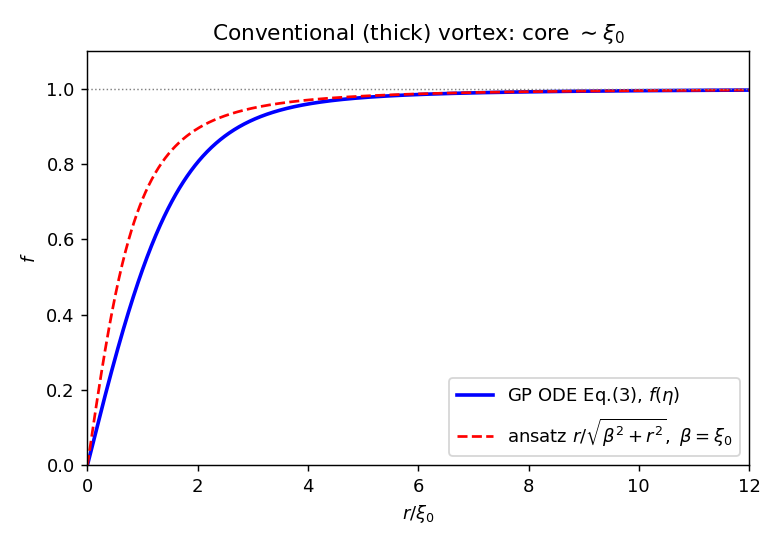
\includegraphics[width=0.48\textwidth]{thick_vortex_profile.png}\hfill
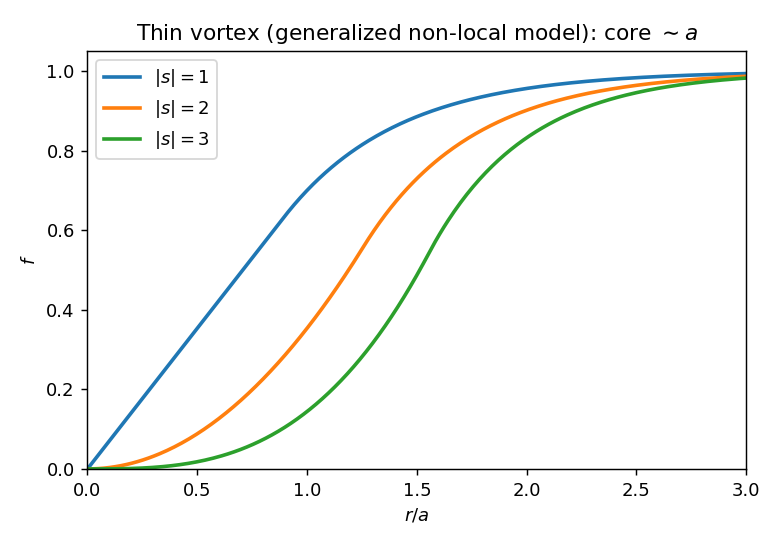
\includegraphics[width=0.48\textwidth]{thin_vortex_profiles.png}
\caption{Left: conventional (thick) vortex $f(\eta)$ from the GP ODE Eq.~3,
core $\sim\xi_0$, with the $r/\sqrt{\beta^2+r^2}$ ansatz ($\beta=\xi_0$) overlaid.
Right: thin-vortex generalized non-local profiles for $|s|=1,2,3$ vs $r/a$,
reproducing paper Fig.~1 --- core $\sim a$.}
\end{figure}
\begin{figure}[h]\centering
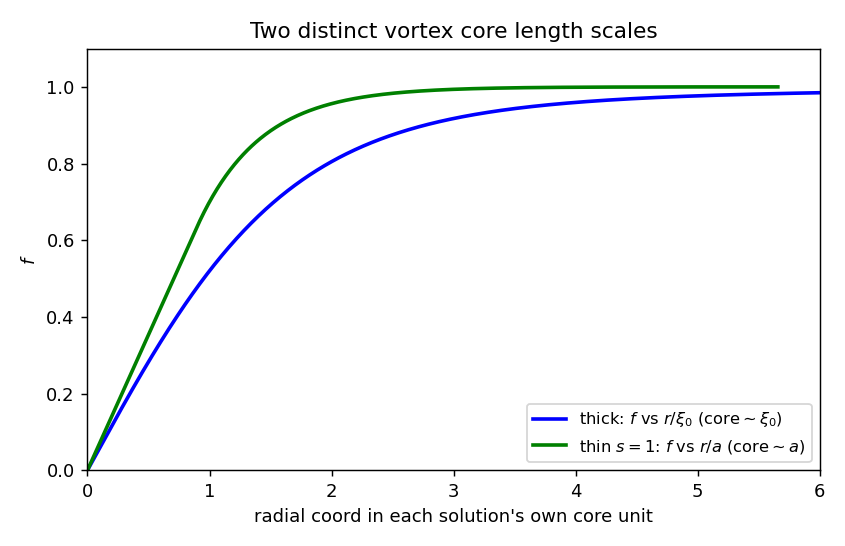
\includegraphics[width=0.48\textwidth]{two_length_scales.png}\hfill
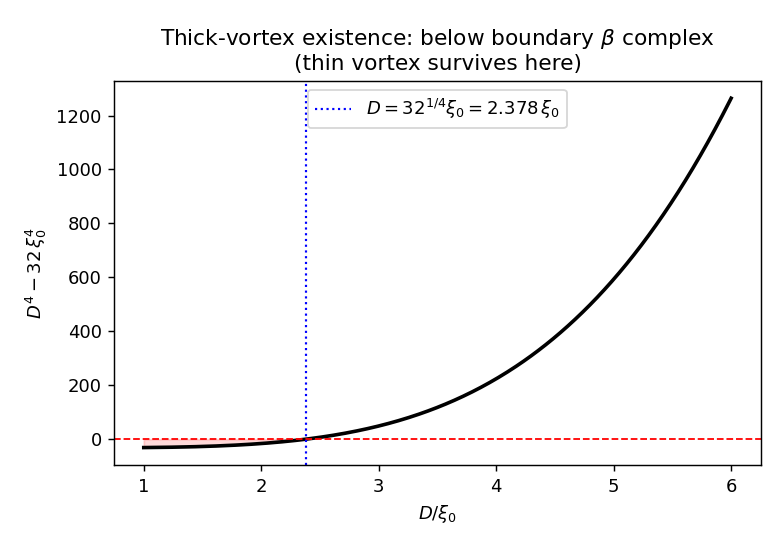
\includegraphics[width=0.48\textwidth]{thick_existence_boundary.png}
\caption{Left: the two solutions plotted each in its own core unit, showing
the microscopic ($a$) vs mesoscopic ($\xi_0$) core scales. Right: the
thick-vortex discriminant $D^4-32\xi_0^4$; below $D=32^{1/4}\xi_0$ it is negative
($\beta$ complex, thick vortex ceases) and only the thin branch survives.}
\end{figure}

\section{Discussion}
Every quantitative and structural claim reproduces to machine precision where a
closed form exists ($\alpha_{s=1}$, $\beta_{\rm thin}$, existence boundary), and
qualitatively where a numerical solve is involved (conventional profile, core
width). The two length scales are demonstrably independent: the thick core is
fixed by $\xi_0$ only (via the local-GP quartic), the thin core by $a$ only (via
the non-local subleading balance, with no $\xi_0$ appearing). The window for
observing the thin vortex --- $\xi_0\sim D$ (equivalently $D^4<32\xi_0^4$), where
the Pad\'e thick solution breaks down --- is reproduced by the discriminant sign
change. \textbf{Verdict: REPLICATED (12/12 claims).}

\end{document}
